\documentclass[aspectratio=169, 10pt, french]{beamer}

% ==============================================================================
% CONFIGURATION PACKAGES & TYPOGRAPHIE
% ==============================================================================
\usepackage[utf8]{inputenc}
\usepackage[T1]{fontenc}
\usepackage{babel}
\usepackage{lmodern}
\usepackage{amsmath,amssymb,amsfonts,amsthm}
\usepackage{graphicx}
\usepackage{booktabs}
\usepackage{tabularx}
\usepackage{array}
\usepackage{tikz}
\usetikzlibrary{shapes.geometric,arrows.meta,positioning,calc,shadows}
\usepackage{tcolorbox}
\tcbuselibrary{skins,breakable}

% ==============================================================================
% PALETTE DE COULEURS DE PRESTIGE (ENSGMM / UNSTIM)
% ==============================================================================
\definecolor{navyblue}{RGB}{26, 54, 93}      % #1A365D - Bleu impérial
\definecolor{royalblue}{RGB}{43, 108, 176}   % #2B6CB0 - Bleu royal moderne
\definecolor{softblue}{RGB}{240, 246, 252}   % Fond bleu très doux
\definecolor{crimsonred}{RGB}{155, 44, 44}   % #9B2C2C - Rouge alerte/virus
\definecolor{goldaccent}{RGB}{214, 158, 46}  % #D69E2E - Liseré or de prestige
\definecolor{darkcharcoal}{RGB}{45, 55, 72}  % #2D3748 - Texte anthracite
\definecolor{cardbg}{RGB}{248, 250, 252}     % Fond de carte
\definecolor{forestgreen}{RGB}{39, 110, 68}  % #276E44 - Vert succès/thérapie

% Configuration Beamer
\usetheme{Boadilla}
\usecolortheme{whale}

\setbeamercolor{structure}{fg=navyblue}
\setbeamercolor{palette primary}{bg=navyblue, fg=white}
\setbeamercolor{palette secondary}{bg=royalblue, fg=white}
\setbeamercolor{palette tertiary}{bg=navyblue!90, fg=white}
\setbeamercolor{title}{bg=navyblue, fg=white}
\setbeamercolor{frametitle}{bg=navyblue, fg=white}
\setbeamercolor{normal text}{fg=darkcharcoal, bg=white}
\setbeamercolor{item}{fg=royalblue}
\setbeamercolor{subitem}{fg=goldaccent}

\setbeamertemplate{navigation symbols}{}

\setbeamerfont{frametitle}{series=\bfseries, size=\large}
\setbeamerfont{title}{series=\bfseries, size=\Large}
\setbeamerfont{subtitle}{series=\normalfont\itshape, size=\small}
\setbeamerfont{footline}{size=\tiny}

\setbeamertemplate{headline}{%
    \leavevmode
    \begin{beamercolorbox}[wd=\paperwidth,ht=2.3ex,dp=0.8ex,leftskip=0.8cm,rightskip=0.8cm]{palette primary}%
        {\tiny\textbf{\textsc{UNSTIM / ENSGMM}} \quad $\bullet$ \quad \textbf{UE : Outils de Calcul Scientifique} \hfill \textcolor{goldaccent}{\textbf{\insertsectionhead}}}%
    \end{beamercolorbox}%
}

\setbeamertemplate{footline}{%
    \leavevmode
    \begin{beamercolorbox}[wd=\paperwidth,ht=2.5ex,dp=1ex,leftskip=0.8cm,rightskip=0.8cm]{palette tertiary}%
        {\tiny\textbf{Groupe 5} (GMM1) \quad $\bullet$ \quad Simulation de Cohorte VIH \& HPC (BLAS/LAPACK/MKL) \hfill \textbf{\insertframenumber{} / \inserttotalframenumber}}%
    \end{beamercolorbox}%
}

% Boîtes d'alerte et de synthèse stylisées
\newtcolorbox{cadreconcept}[1][]{
    colback=softblue,
    colframe=navyblue,
    arc=3pt,
    boxrule=0.8pt,
    fonttitle=\bfseries\color{white},
    coltitle=white,
    title=#1,
    top=3pt, bottom=3pt, left=6pt, right=6pt
}

\newtcolorbox{cadrehpc}[1][]{
    colback=cardbg,
    colframe=royalblue,
    arc=3pt,
    boxrule=0.8pt,
    fonttitle=\bfseries\color{white},
    coltitle=white,
    title=#1,
    top=3pt, bottom=3pt, left=6pt, right=6pt
}

\newtcolorbox{cadreclinique}[1][]{
    colback=red!5!white,
    colframe=crimsonred,
    arc=3pt,
    boxrule=0.8pt,
    fonttitle=\bfseries\color{white},
    coltitle=white,
    title=#1,
    top=3pt, bottom=3pt, left=6pt, right=6pt
}

% Métadonnées
\title[\textbf{Modèle Cohorte VIH \& HPC}]{\textbf{Modélisation Multi-Patient de l'Infection VIH-SIDA et Analyse Pronostique Haute Performance}}
\subtitle{Formulation Matricielle BLAS 3, Décomposition de Cholesky LAPACK et Accélération Intel oneMKL}
\author[\textbf{Groupe 5 -- ENSGMM1}]{\textbf{Groupe 5 :}\\[0.05cm] \textbf{ADOGOUN Déo Gracias M.} \quad $\bullet$ \quad \textbf{BIAHOU Ahossou J. M.-C.} \quad $\bullet$ \quad \textbf{SYLLA IMOROU Izou Dine}}
\institute[\textbf{ENSGMM / UNSTIM}]{\textbf{ENSGMM -- UNSTIM Abomey} \quad $\bullet$ \quad \textbf{Sous la direction de : Dr. Carlos AGOSSOU}}
\date{\textbf{Année académique 2026--2027}}

\graphicspath{{figures/}{../figures/}{docs/figures/}}

\begin{document}

% ------------------------------------------------------------------------------
% 1. PAGE DE GARDE INSTITUTIONNELLE
% ------------------------------------------------------------------------------
\begin{frame}[plain]
    \begin{tikzpicture}[remember picture, overlay]
        \fill[white] (current page.north west) rectangle (current page.south east);
        \draw[line width=1.6pt, color=navyblue] 
            ($(current page.north west) + (0.45cm,-0.45cm)$) rectangle 
            ($(current page.south east) + (-0.45cm,0.45cm)$);
        \draw[line width=0.6pt, color=goldaccent] 
            ($(current page.north west) + (0.55cm,-0.55cm)$) rectangle 
            ($(current page.south east) + (-0.55cm,0.55cm)$);
    \end{tikzpicture}

    \centering
    \vspace*{0.4cm}

    % Logos institutionnels
    \begin{columns}[c]
        \begin{column}{0.18\textwidth}
            \centering
            
\includegraphics[height=1.30cm, keepaspectratio]{logo_unstim.png}
        \end{column}
        \begin{column}{0.64\textwidth}
            \centering
            {\scriptsize \textsc{\textbf{République du Bénin}}}\\[0.02cm]
            {\tiny \textbf{Ministère de l'Enseignement Supérieur et de la Recherche Scientifique}}\\[0.04cm]
            {\scriptsize \textbf{UNIVERSITÉ NATIONALE DES SCIENCES, TECHNOLOGIES,}}\\[0.02cm]
            {\scriptsize \textbf{INGÉNIERIE ET MATHÉMATIQUES D'ABOMEY (UNSTIM)}}\\[0.04cm]
            {\footnotesize \textcolor{navyblue}{\textbf{ÉCOLE NATIONALE SUPÉRIEURE DE GÉNIE MATHÉMATIQUE ET MODÉLISATION (ENSGMM)}}}
        \end{column}
        \begin{column}{0.18\textwidth}
            \centering
            
\includegraphics[height=1.30cm, keepaspectratio]{logo_ensgmm.png}
        \end{column}
    \end{columns}

    \vspace{0.10cm}
    \textcolor{goldaccent}{\rule{0.85\textwidth}{1.0pt}}
    \vspace{0.10cm}

    % Titre principal
    \begin{tcolorbox}[
        colback=navyblue,
        colframe=navyblue,
        arc=4pt,
        boxrule=0pt,
        width=0.96\textwidth,
        halign=center,
        top=4pt, bottom=4pt
    ]
        {\large\bfseries\color{white} Modélisation Multi-Patient de l'Infection VIH-SIDA}\\[0.08cm]
        {\small\color{goldaccent}\textit{Formulation Matricielle BLAS 3, Résolution de Cholesky LAPACK}}\\[0.03cm]
        {\small\color{goldaccent}\textit{et Accélération Haute Performance avec Intel oneMKL en Python}}
    \end{tcolorbox}

    \vspace{0.10cm}

    % Groupe et encadrement
    \begin{tcolorbox}[
        colback=cardbg,
        colframe=gray!30,
        arc=3pt,
        boxrule=0.6pt,
        width=0.96\textwidth,
        top=3pt, bottom=3pt
    ]
        \centering
        {\footnotesize \textbf{\textcolor{navyblue}{\underline{Équipe de Projet -- Groupe 5 :}}}}\\[0.05cm]
        {\footnotesize \textbf{ADOGOUN Déo Gracias M.} \quad $\bullet$ \quad \textbf{BIAHOU Ahossou J. M.-C.} \quad $\bullet$ \quad \textbf{SYLLA IMOROU Izou Dine}}\\[0.08cm]
        {\scriptsize Filière : ENSGMM 1 \quad $\bullet$ \quad UE : Outils de Calcul Scientifique \quad $\bullet$ \quad Promotion 2025--2026}\\[0.04cm]
        {\scriptsize \textbf{Sous la direction de : \textcolor{navyblue}{Dr. Carlos AGOSSOU}}}
    \end{tcolorbox}
\end{frame}

% ------------------------------------------------------------------------------
% 2. PLAN DE LA SOUTENANCE
% ------------------------------------------------------------------------------
\section{Plan Général}
\begin{frame}{Plan de la Soutenance}
    \begin{columns}[t]
        \begin{column}{0.48\textwidth}
            \begin{cadreconcept}[\textbf{1. Contexte Biomédical \& Enjeu HPC}]
                \small
                \begin{itemize}
                    \item Suivi de cohortes massives de patients ($N \ge 10\,000$)
                    \item Inefficacité du calcul scalaire en Python pur
                    \item Nécessité de BLAS, LAPACK et Intel oneMKL
                \end{itemize}
            \end{cadreconcept}
            \vspace{0.15cm}
            \begin{cadreconcept}[\textbf{2. Modèle de Cohorte \& Résistance}]
                \small
                \begin{itemize}
                    \item 5 compartiments : $T$, $I_s$, $I_r$, $V_s$, $V_r$
                    \item Taux de mutation $\mu$ et multithérapie ART
                    \item Émergence du rebond viral résistant
                \end{itemize}
            \end{cadreconcept}
        \end{column}

        \begin{column}{0.48\textwidth}
            \begin{cadrehpc}[\textbf{3. Formulation Matricielle \& BLAS 3}]
                \small
                \begin{itemize}
                    \item Matrice d'état de cohorte $\mathbf{Y} \in \mathbb{R}^{N \times 5}$
                    \item Équation vectorielle $\dot{\mathbf{Y}} = \mathbf{S} + \mathbf{Y}\mathbf{M}^T + \mathbf{\Phi}\mathbf{A}^T$
                    \item Intégrateur Runge-Kutta 4 par \texttt{DGEMM}
                \end{itemize}
            \end{cadrehpc}
            \vspace{0.15cm}
            \begin{cadrehpc}[\textbf{4. Analyse LAPACK \& Benchmarks}]
                \small
                \begin{itemize}
                    \item Régression Ridge via Cholesky (\texttt{DPOTRF/DPOTRS})
                    \item Stratification ACP Divide \& Conquer (\texttt{DSYEVD})
                    \item Bancs d'essai : Naïf vs MKL, Scalabilité OpenMP
                \end{itemize}
            \end{cadrehpc}
        \end{column}
    \end{columns}
\end{frame}

% ------------------------------------------------------------------------------
% 3. PROBLEMATIQUE BIOMEDICALE ET HPC
% ------------------------------------------------------------------------------
\section{Contexte \& Enjeu HPC}
\begin{frame}{Le Défi : Modéliser une Cohorte Clinique Massive}
    \begin{columns}[c]
        \begin{column}{0.52\textwidth}
            \begin{cadreclinique}[\textbf{La Réalité Clinique du VIH}]
                \small
                \begin{itemize}
                    \item Dans un hôpital ou un essai clinique, on ne traite pas un patient isolé, mais des \textbf{cohortes de milliers d'individus}.
                    \item \textbf{Hétérogénéité biologique} : chaque patient possède sa propre charge initiale, son taux d'adhésion au traitement $\eta_k$, et sa sensibilité.
                    \item \textbf{Phénomène d'échappement} : sous traitement incomplet, une souche virale mutante résistante émerge et provoque le rebond viral.
                \end{itemize}
            \end{cadreclinique}
        \end{column}

        \begin{column}{0.48\textwidth}
            \begin{cadrehpc}[\textbf{Le Piège du Calcul Naïf}]
                \small
                \begin{itemize}
                    \item Simuler $N = 10\,000$ patients sur 365 jours par une boucle Python :
                    $$\text{Temps} \approx N \times \text{Nsteps} \times \text{Overhead CPython}$$
                    \item Les boucles interprétées en Python pur subissent un surcoût colossal de typage dynamique et de cache miss.
                    \item \textbf{Solution} : Traiter l'ensemble de la cohorte comme un \textbf{tenseur matriciel continu} exploité par des routines compilées ultra-optimisées.
                \end{itemize}
            \end{cadrehpc}
        \end{column}
    \end{columns}
\end{frame}

% ------------------------------------------------------------------------------
% 4. HIERARCHIE BLAS ET INTEL MKL
% ------------------------------------------------------------------------------
\begin{frame}{La Hiérarchie BLAS et l'Avantage BLAS 3}
    \begin{center}
    \small
    \begin{tabularx}{\textwidth}{lccccX}
        \toprule
        \textbf{Niveau} & \textbf{Opération Type} & \textbf{Mémoire} & \textbf{Flops} & \textbf{Ratio $q$} & \textbf{Comportement Matériel} \\
        \midrule
        \textbf{BLAS 1} & $\mathbf{y} \leftarrow \alpha\mathbf{x} + \mathbf{y}$ (\texttt{DAXPY}) & $3n$ & $2n$ & $\mathcal{O}(1)$ & Limité par la bande passante RAM \\
        \textbf{BLAS 2} & $\mathbf{y} \leftarrow \alpha\mathbf{A}\mathbf{x} + \beta\mathbf{y}$ (\texttt{DGEMV}) & $n^2$ & $2n^2$ & $\mathcal{O}(1)$ & Saturation rapide du bus mémoire \\
        \textbf{BLAS 3} & $\mathbf{C} \leftarrow \alpha\mathbf{A}\mathbf{B} + \beta\mathbf{C}$ (\texttt{DGEMM}) & $3n^2$ & $2n^3$ & $\mathcal{O}(n)$ & \textbf{Calcul arithmétique pur en cache L1/L2} \\
        \bottomrule
    \end{tabularx}
    \end{center}

    \vspace{0.2cm}
    \begin{columns}[c]
        \begin{column}{0.50\textwidth}
            \begin{cadrehpc}[\textbf{Le Mur de la Mémoire (\textit{Memory Wall})}]
                \footnotesize
                La vitesse des processeurs a crû bien plus vite que la bande passante mémoire.
                Pour atteindre les performances crêtes (GFLOPS), une routine doit \textbf{réutiliser les données en cache} : c'est l'essence même de BLAS 3.
            \end{cadrehpc}
        \end{column}
        \begin{column}{0.50\textwidth}
            \begin{cadreconcept}[\textbf{Intel oneMKL (Math Kernel Library)}]
                \footnotesize
                Bibliothèque hautement optimisée pour architectures Intel/AMD :
                \begin{itemize}
                    \item Vectorisation matérielle SIMD (AVX-2, AVX-512).
                    \item Parallélisme multi-cœurs OpenMP transparent.
                    \item Micro-noyaux de partitionnement de cache par blocs.
                \end{itemize}
            \end{cadreconcept}
        \end{column}
    \end{columns}
\end{frame}

% ------------------------------------------------------------------------------
% 5. LE MODELE DE COHORTE MATHEMATIQUE
% ------------------------------------------------------------------------------
\section{Modèle Biomathématique}
\begin{frame}{Le Modèle de Cohorte avec Émergence de Résistance}
    Pour chaque patient $k \in \{1, \dots, N\}$, l'état viral et immunitaire est décrit par 5 compartiments :
    \begin{align*}
        \frac{dT_k}{dt} &= s - d\,T_k - (1 - \eta_{s,k})\,\beta_s\,T_k\,V_{s,k} - (1 - \eta_{r,k})\,\beta_r\,T_k\,V_{r,k} \\
        \frac{dI_{s,k}}{dt} &= (1 - \mu)\,(1 - \eta_{s,k})\,\beta_s\,T_k\,V_{s,k} - \delta\,I_{s,k} \\
        \frac{dI_{r,k}}{dt} &= \mu\,(1 - \eta_{s,k})\,\beta_s\,T_k\,V_{s,k} + (1 - \eta_{r,k})\,\beta_r\,T_k\,V_{r,k} - \delta\,I_{r,k} \\
        \frac{dV_{s,k}}{dt} &= p\,I_{s,k} - c\,V_{s,k} \\
        \frac{dV_{r,k}}{dt} &= p\,I_{r,k} - c\,V_{r,k}
    \end{align*}

    \begin{cadreclinique}[\textbf{Mécanisme Clé : Mutation et Pression Thérapeutique}]
        \footnotesize
        \begin{itemize}
            \item $\mu = 10^{-4}$ : Taux de mutation ponctuelle lors de la transcription inverse.
            \item Le traitement ART cible la souche sauvage avec l'efficacité $\eta_{s,k} \in [0.50, 0.95]$.
            \item La souche mutante échappe en partie au traitement : $\eta_{r,k} = \max(0, \eta_{s,k} - 0.35)$.
        \end{itemize}
    \end{cadreclinique}
\end{frame}

% ------------------------------------------------------------------------------
% 6. FORMULATION MATRICIELLE GLOBALE
% ------------------------------------------------------------------------------
\section{Formulation Matricielle \& BLAS 3}
\begin{frame}{Formulation Matricielle Globale pour $N$ Patients}
    On rassemble l'ensemble de la cohorte dans une matrice d'état continue $\mathbf{Y} \in \mathbb{R}^{N \times 5}$ :
    $$\mathbf{Y} = \begin{pmatrix} T_1 & I_{s,1} & I_{r,1} & V_{s,1} & V_{r,1} \\ \vdots & \vdots & \vdots & \vdots & \vdots \\ T_N & I_{s,N} & I_{r,N} & V_{s,N} & V_{r,N} \end{pmatrix}$$

    Le système de $5N$ équations différentielles se condense en une \textbf{unique équation différentielle matricielle} :
    \begin{equation*}
        \mathbf{\dot{Y}} = \mathbf{S} + \mathbf{Y}\,\mathbf{M}^T + \mathbf{\Phi}\,\mathbf{A}^T
    \end{equation*}

    \begin{columns}[t]
        \begin{column}{0.48\textwidth}
            \begin{cadrehpc}[\textbf{Partie Linéaire : $\mathbf{M} \in \mathbb{R}^{5 \times 5}$}]
                \footnotesize
                $$\mathbf{M} = \begin{pmatrix}
                -d & 0 & 0 & 0 & 0 \\
                0 & -\delta & 0 & 0 & 0 \\
                0 & 0 & -\delta & 0 & 0 \\
                0 & p & 0 & -c & 0 \\
                0 & 0 & p & 0 & -c
                \end{pmatrix}$$
                Terme source : $\mathbf{S} = \mathbf{1}_N \otimes (s, 0, 0, 0, 0)$.
            \end{cadrehpc}
        \end{column}

        \begin{column}{0.48\textwidth}
            \begin{cadrehpc}[\textbf{Partie Non-Linéaire : $\mathbf{\Phi} \in \mathbb{R}^{N \times 2}$}]
                \footnotesize
                Flux d'infections sensibles et mutantes :
                $$\mathbf{\Phi}_{k,0} = (1 - \eta_{s,k})\beta_s T_k V_{s,k}$$
                $$\mathbf{\Phi}_{k,1} = (1 - \eta_{r,k})\beta_r T_k V_{r,k}$$
                Matrice stœchiométrique $\mathbf{A} \in \mathbb{R}^{5 \times 2}$ :
                $$\mathbf{A}^T = \begin{pmatrix} -1 & -1 \\ 1-\mu & 0 \\ \mu & 1 \\ 0 & 0 \\ 0 & 0 \end{pmatrix}^T$$
            \end{cadrehpc}
        \end{column}
    \end{columns}
\end{frame}

% ------------------------------------------------------------------------------
% 7. INTEGRATION TEMPORELLE RK4 PAR BLAS 3
% ------------------------------------------------------------------------------
\begin{frame}{Intégration Temporelle Runge-Kutta 4 par Micro-Noyaux BLAS 3}
    L'évaluation du second membre $\mathbf{F}(\mathbf{Y}) = \mathbf{S} + \mathbf{Y}\,\mathbf{M}^T + \mathbf{\Phi}\,\mathbf{A}^T$ fait intervenir deux produits matriciels :
    \begin{itemize}
        \item $\mathbf{Y}\,\mathbf{M}^T$ avec $\mathbf{Y} \in \mathbb{R}^{N \times 5}$ et $\mathbf{M}^T \in \mathbb{R}^{5 \times 5}$ : appel BLAS 3 \texttt{DGEMM}.
        \item $\mathbf{\Phi}\,\mathbf{A}^T$ avec $\mathbf{\Phi} \in \mathbb{R}^{N \times 2}$ et $\mathbf{A}^T \in \mathbb{R}^{2 \times 5}$ : appel BLAS 3 \texttt{DGEMM}.
    \end{itemize}

    \begin{cadrehpc}[\textbf{Algorithme Vectorisé RK4 pour la Cohorte}]
        \small
        À chaque pas de temps $h$ pour toute la cohorte simultanément :
        \begin{align*}
            \mathbf{K}_1 &= \mathbf{F}(\mathbf{Y}_n) \\
            \mathbf{K}_2 &= \mathbf{F}\left(\mathbf{Y}_n + \frac{h}{2}\mathbf{K}_1\right) \\
            \mathbf{K}_3 &= \mathbf{F}\left(\mathbf{Y}_n + \frac{h}{2}\mathbf{K}_2\right) \\
            \mathbf{K}_4 &= \mathbf{F}(\mathbf{Y}_n + h\,\mathbf{K}_3) \\
            \mathbf{Y}_{n+1} &= \mathbf{Y}_n + \frac{h}{6}\left(\mathbf{K}_1 + 2\mathbf{K}_2 + 2\mathbf{K}_3 + \mathbf{K}_4\right)
        \end{align*}
        \textbf{Avantage majeur} : Zéro boucle Python sur les patients. La totalité du calcul est traitée en mémoire C/Fortran contiguë dans les registres vectoriels SIMD !
    \end{cadrehpc}
\end{frame}

% ------------------------------------------------------------------------------
% 8. ANALYSE CLINIQUE PAR CHOLESKY LAPACK
% ------------------------------------------------------------------------------
\section{Analyse Clinique LAPACK}
\begin{frame}{Analyse Clinique Pronostique : Régression Ridge via LAPACK}
    \begin{columns}[c]
        \begin{column}{0.50\textwidth}
            \begin{cadreclinique}[\textbf{Objectif Médical}]
                \small
                Prédire la charge virale finale d'un patient à partir de ses biomarqueurs à $t = 30$ jours ($T_{30}, V_{s,30}, V_{r,30}, \eta_s$).
                \textbf{Problème} : Les variables sont fortement colinéaires $\implies$ risque d'instabilité numérique.
            \end{cadreclinique}
            \vspace{0.1cm}
            \begin{cadreconcept}[\textbf{Régularisation de Tikhonov (Ridge)}]
                \small
                On résout le système régularisé :
                $$(\mathbf{X}^T\mathbf{X} + \lambda\mathbf{I})\,\mathbf{w} = \mathbf{X}^T\mathbf{y}$$
                La matrice $\mathbf{A}_{\text{ridge}} = \mathbf{X}^T\mathbf{X} + \lambda\mathbf{I}$ est \textbf{symétrique définie positive}.
            \end{cadreconcept}
        \end{column}

        \begin{column}{0.50\textwidth}
            \begin{cadrehpc}[\textbf{Résolution Haute Performance par LAPACK}]
                \small
                \begin{enumerate}
                    \item \textbf{BLAS 3 \texttt{DSYRK}} :
                    Calcul du produit symétrique rang-$k$ :
                    $$\mathbf{C} \leftarrow \mathbf{X}^T\mathbf{X} + \lambda\mathbf{I}$$
                    (2 fois moins d'opérations qu'un produit général).
                    \item \textbf{LAPACK \texttt{DPOTRF}} :
                    Factorisation de Cholesky $\mathbf{A} = \mathbf{L}\mathbf{L}^T$.
                    \item \textbf{LAPACK \texttt{DPOTRS}} :
                    Double descente-remontée triangulaire pour obtenir le vecteur de poids $\mathbf{w}$.
                \end{enumerate}
                \textbf{Gain} : 2 fois plus rapide que la factorisation LU (\texttt{DGESV}) et infiniment plus stable que l'inversion naïve $\mathbf{A}^{-1}$.
            \end{cadrehpc}
        \end{column}
    \end{columns}
\end{frame}

% ------------------------------------------------------------------------------
% 9. STRATIFICATION DES PATIENTS PAR ACP LAPACK
% ------------------------------------------------------------------------------
\begin{frame}{Stratification des Patients par ACP (\texttt{DSYEVD})}
    \begin{columns}[c]
        \begin{column}{0.52\textwidth}
            \begin{cadreconcept}[\textbf{Analyse en Composantes Principales (ACP)}]
                \small
                \begin{itemize}
                    \item Réduction dimensionnelle des profils cliniques de $5$ variables vers les $2$ axes de variance maximale.
                    \item Matrice de covariance empirique $\mathbf{\Sigma} = \frac{1}{N-1}\mathbf{\tilde{X}}^T\mathbf{\tilde{X}} \in \mathbb{R}^{5 \times 5}$ symétrique semi-définie positive.
                    \item Résolution du problème aux valeurs propres :
                    $$\mathbf{\Sigma}\,\mathbf{v}_i = \lambda_i\,\mathbf{v}_i$$
                \end{itemize}
            \end{cadreconcept}
        \end{column}

        \begin{column}{0.48\textwidth}
            \begin{cadrehpc}[\textbf{Routine LAPACK \texttt{DSYEVD}}]
                \small
                \begin{itemize}
                    \item Algorithme de type \textbf{Divide \& Conquer} pour matrices symétriques réelles.
                    \item Complexité réduite et orthogonalité parfaite des vecteurs propres garanties par construction.
                    \item Projection directe des $N$ patients :
                    $$\mathbf{Z} = \mathbf{\tilde{X}}\,\mathbf{V}_{[:, :2]} \in \mathbb{R}^{N \times 2}$$
                    réalisée par BLAS 3 \texttt{DGEMM}.
                \end{itemize}
            \end{cadrehpc}
        \end{column}
    \end{columns}
\end{frame}

% ------------------------------------------------------------------------------
% 10. RESULTATS DE SIMULATION : TRAJECTOIRES DE COHORTE
% ------------------------------------------------------------------------------
\section{Résultats Scientifiques \& HPC}
\begin{frame}{Trajectoires de Cohorte : Répression vs Rebond Mutant}
    \begin{center}
        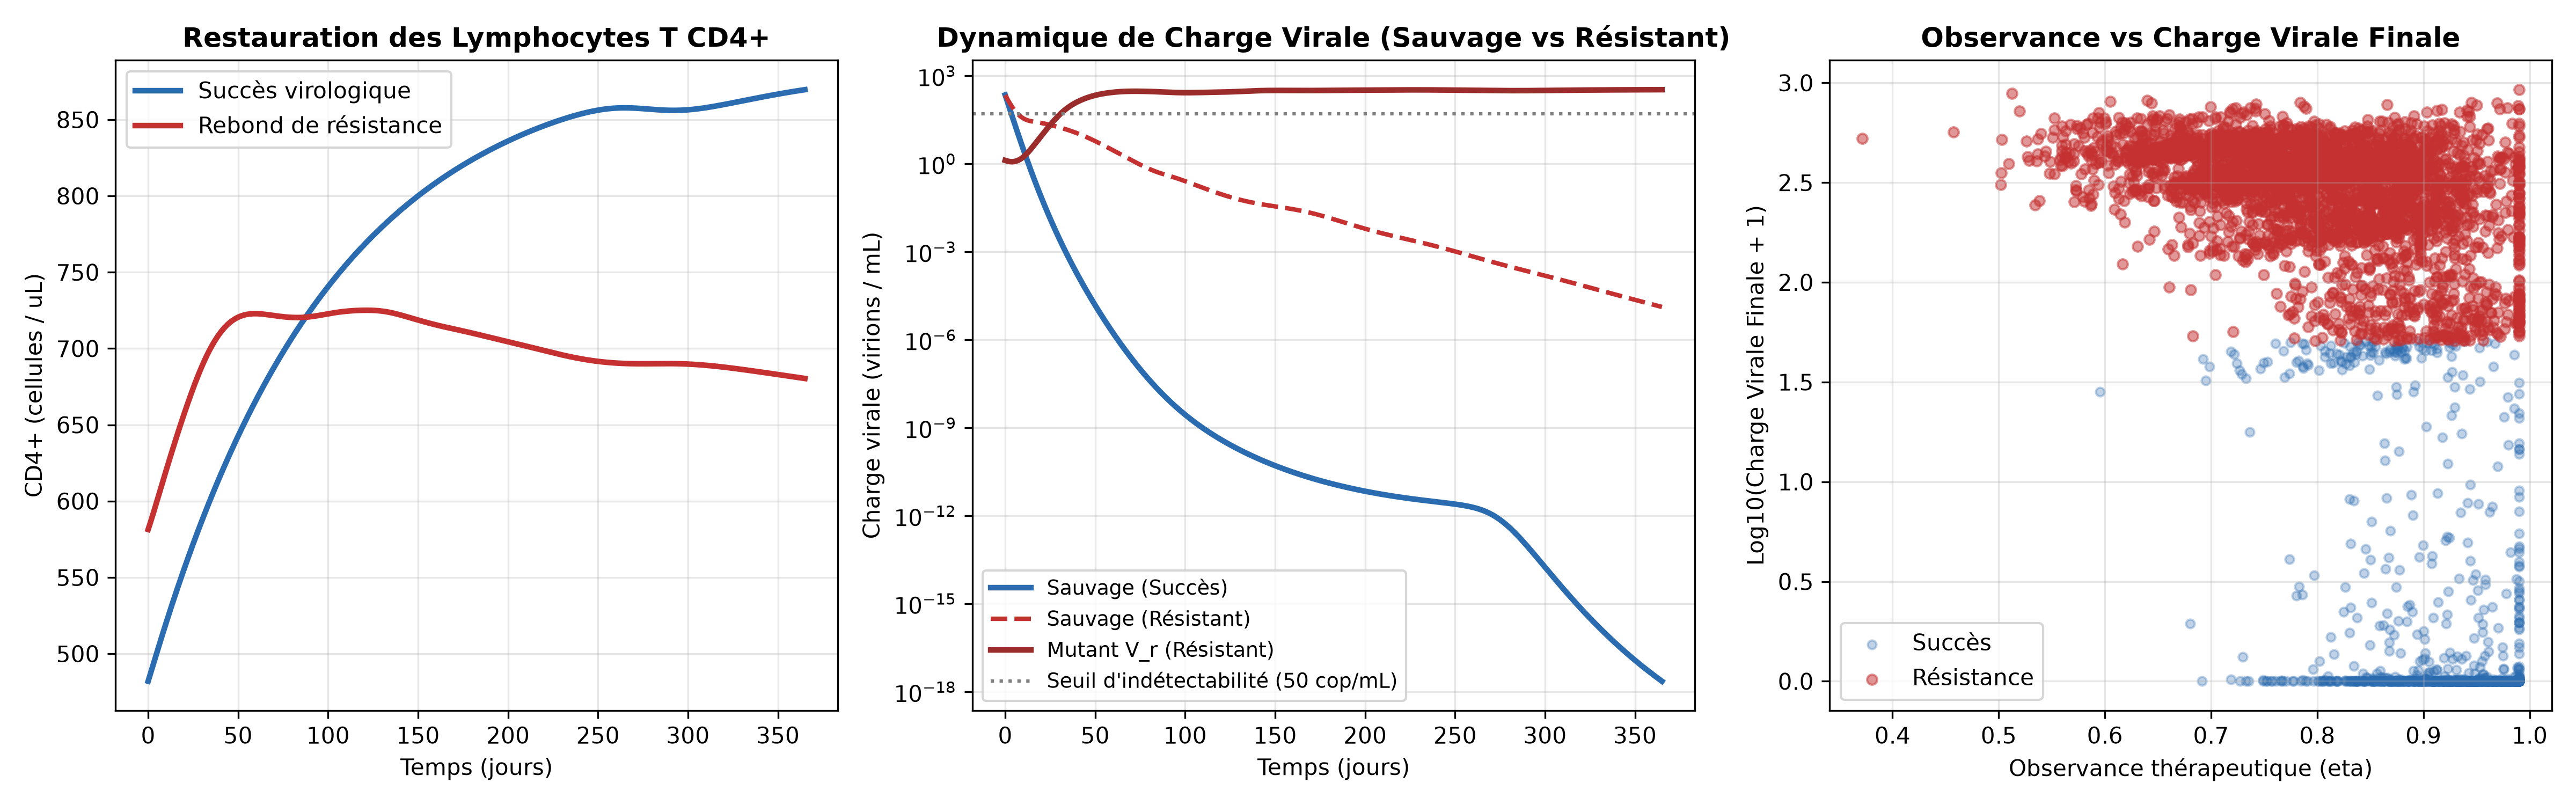
\includegraphics[width=0.88\textwidth, height=5.2cm, keepaspectratio]{cohort_trajectories.png}
    \end{center}
    \footnotesize
    \textbf{Lecture biomédicale} : Sur 5 000 patients simulés pendant 365 jours, le traitement bloque la souche sauvage (bleu). Cependant, les patients avec faible adhésion ($\eta_s < 0.70$) développent la souche résistante (rouge) qui provoque l'effondrement des lymphocytes T CD4+ (vert).
\end{frame}

% ------------------------------------------------------------------------------
% 11. RESULTATS DE STRATIFICATION PAR CLUSTERS PCA
% ------------------------------------------------------------------------------
\begin{frame}{Stratification Clinique des Patients par ACP}
    \begin{center}
        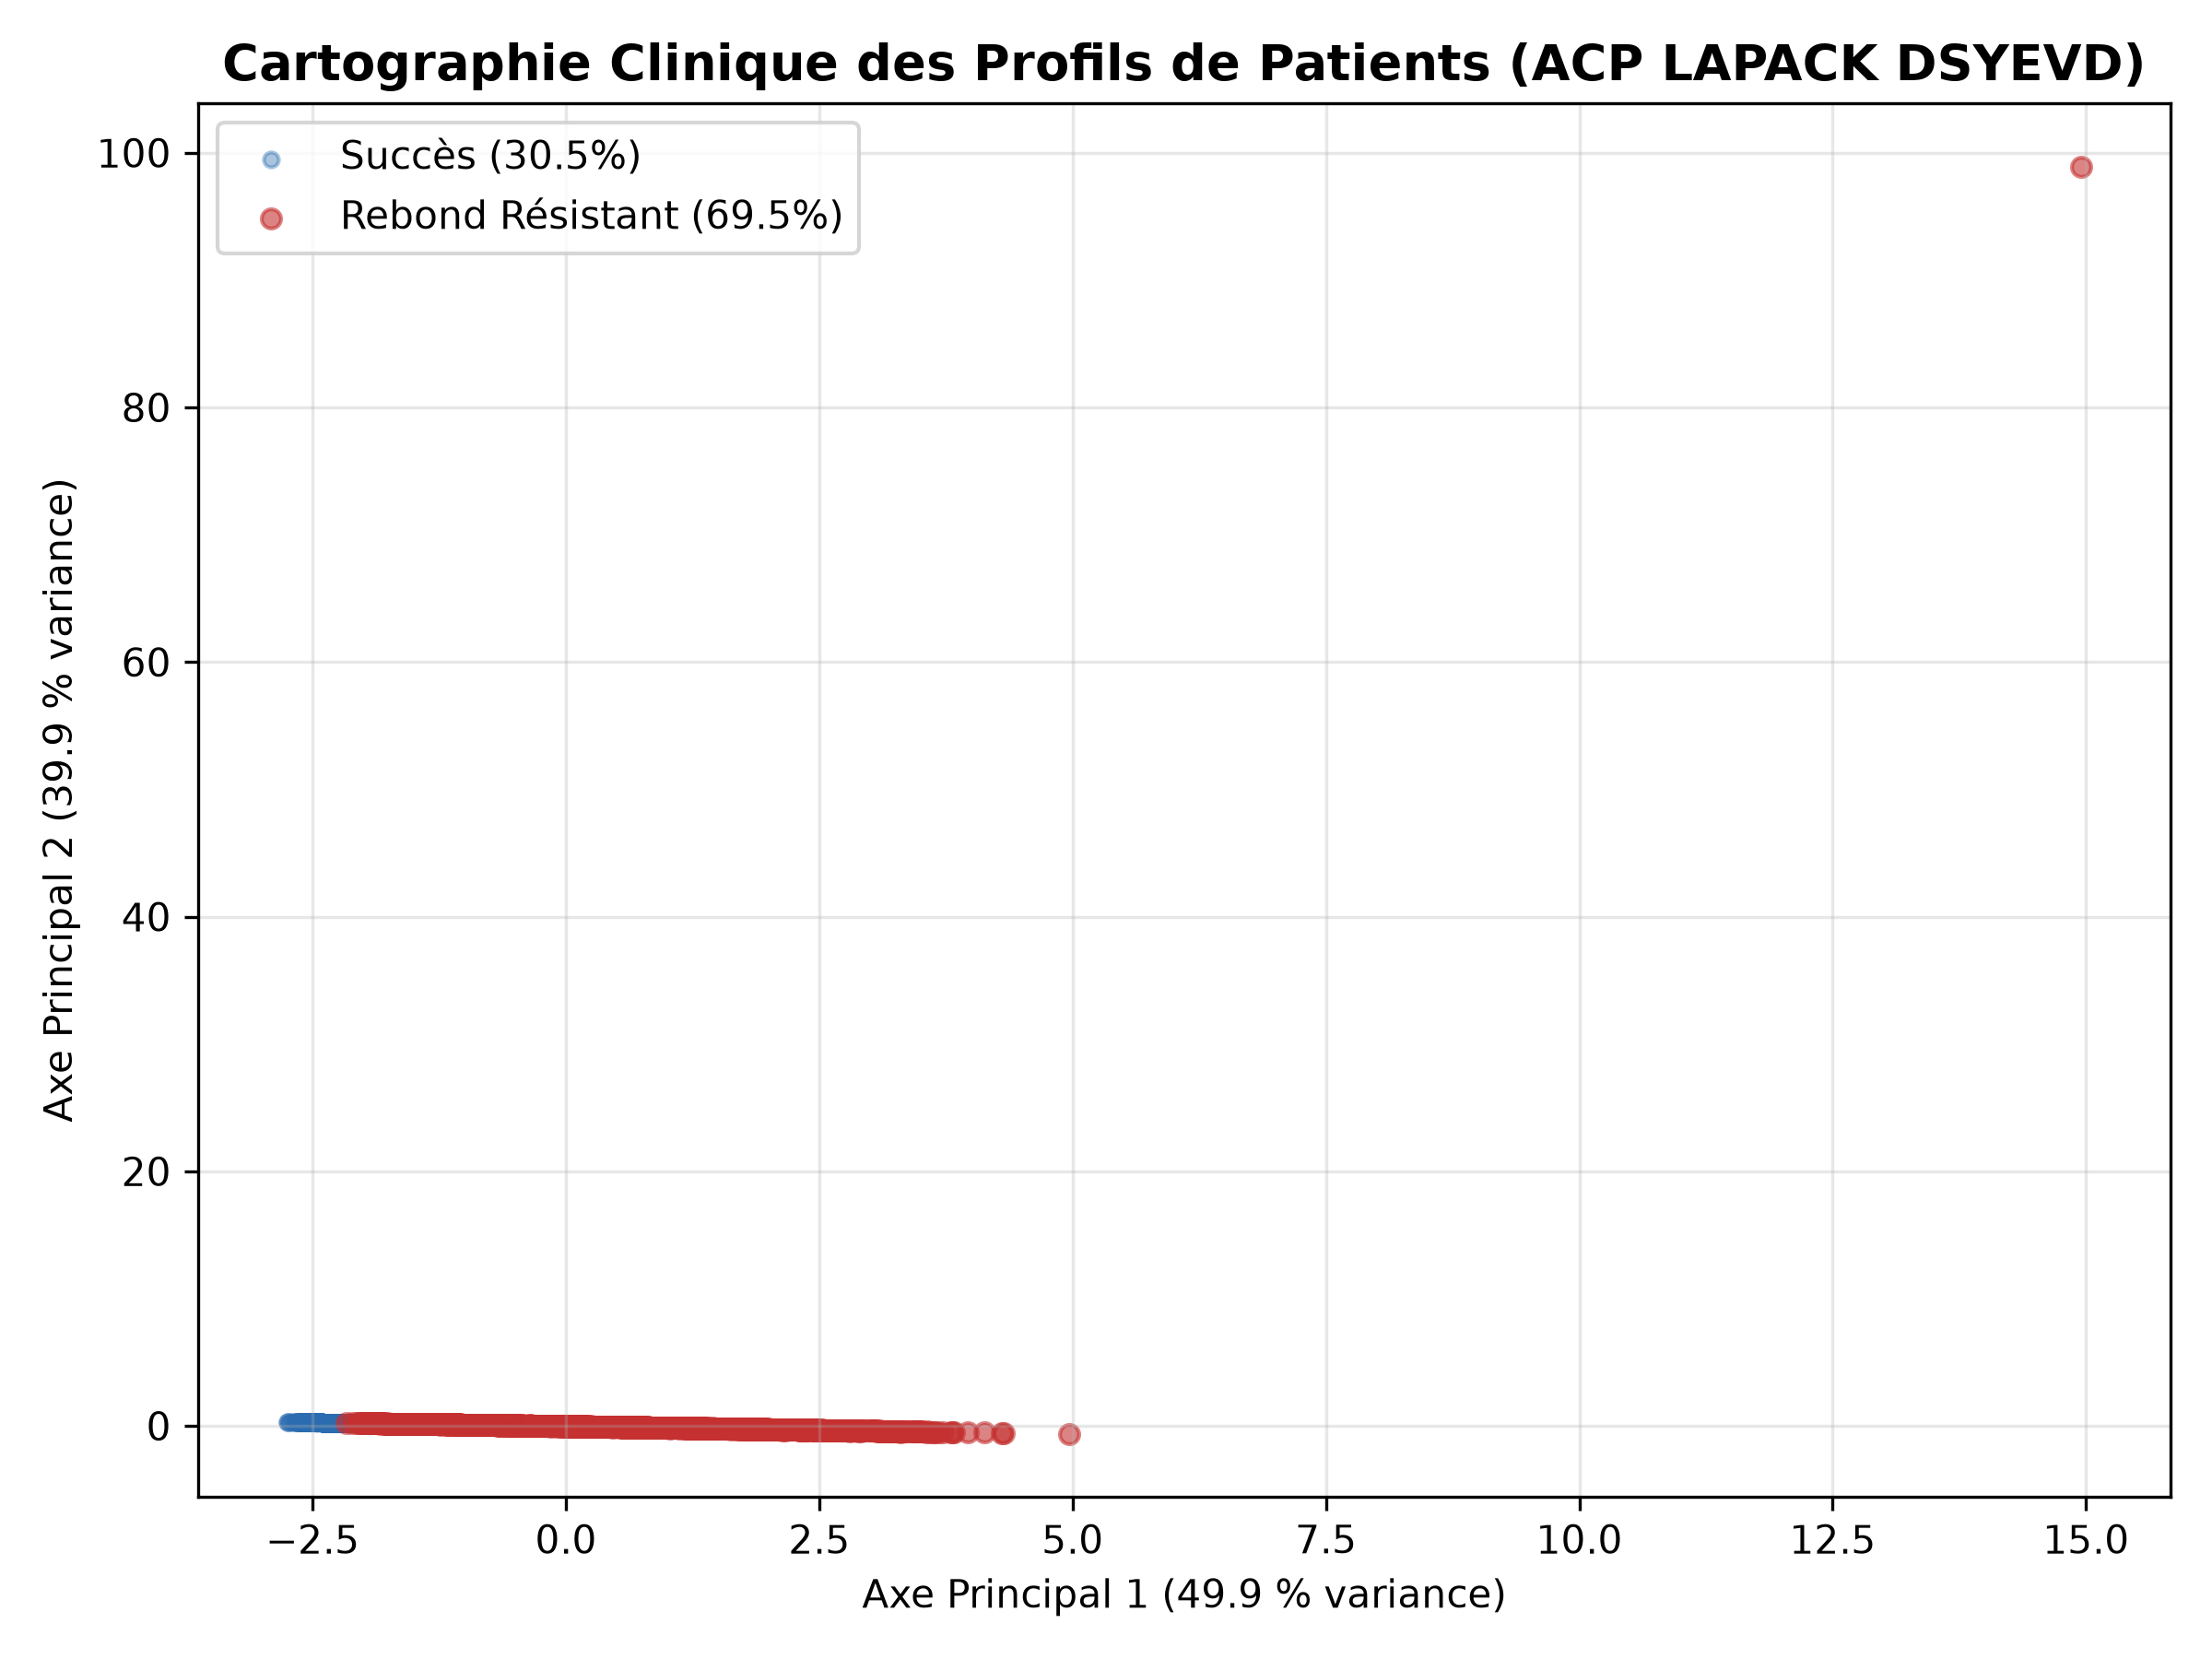
\includegraphics[width=0.62\textwidth, height=5.0cm, keepaspectratio]{clinical_pca_clusters.png}
    \end{center}
    \footnotesize
    \textbf{Visualisation dans le premier plan factoriel} : La première composante (axe horizontal, inertie maximale) sépare nettement les patients répondeurs (contrôle virologique, vert) des patients en échec thérapeutique avec sélection de mutants (rouge).
\end{frame}

% ------------------------------------------------------------------------------
% 12. BENCHMARKS : PYTHON NAIF VS BLAS 3 / MKL
% ------------------------------------------------------------------------------
\begin{frame}{Banc d'Essai : Python Naïf vs BLAS 3 (Intel oneMKL)}
    \begin{center}
        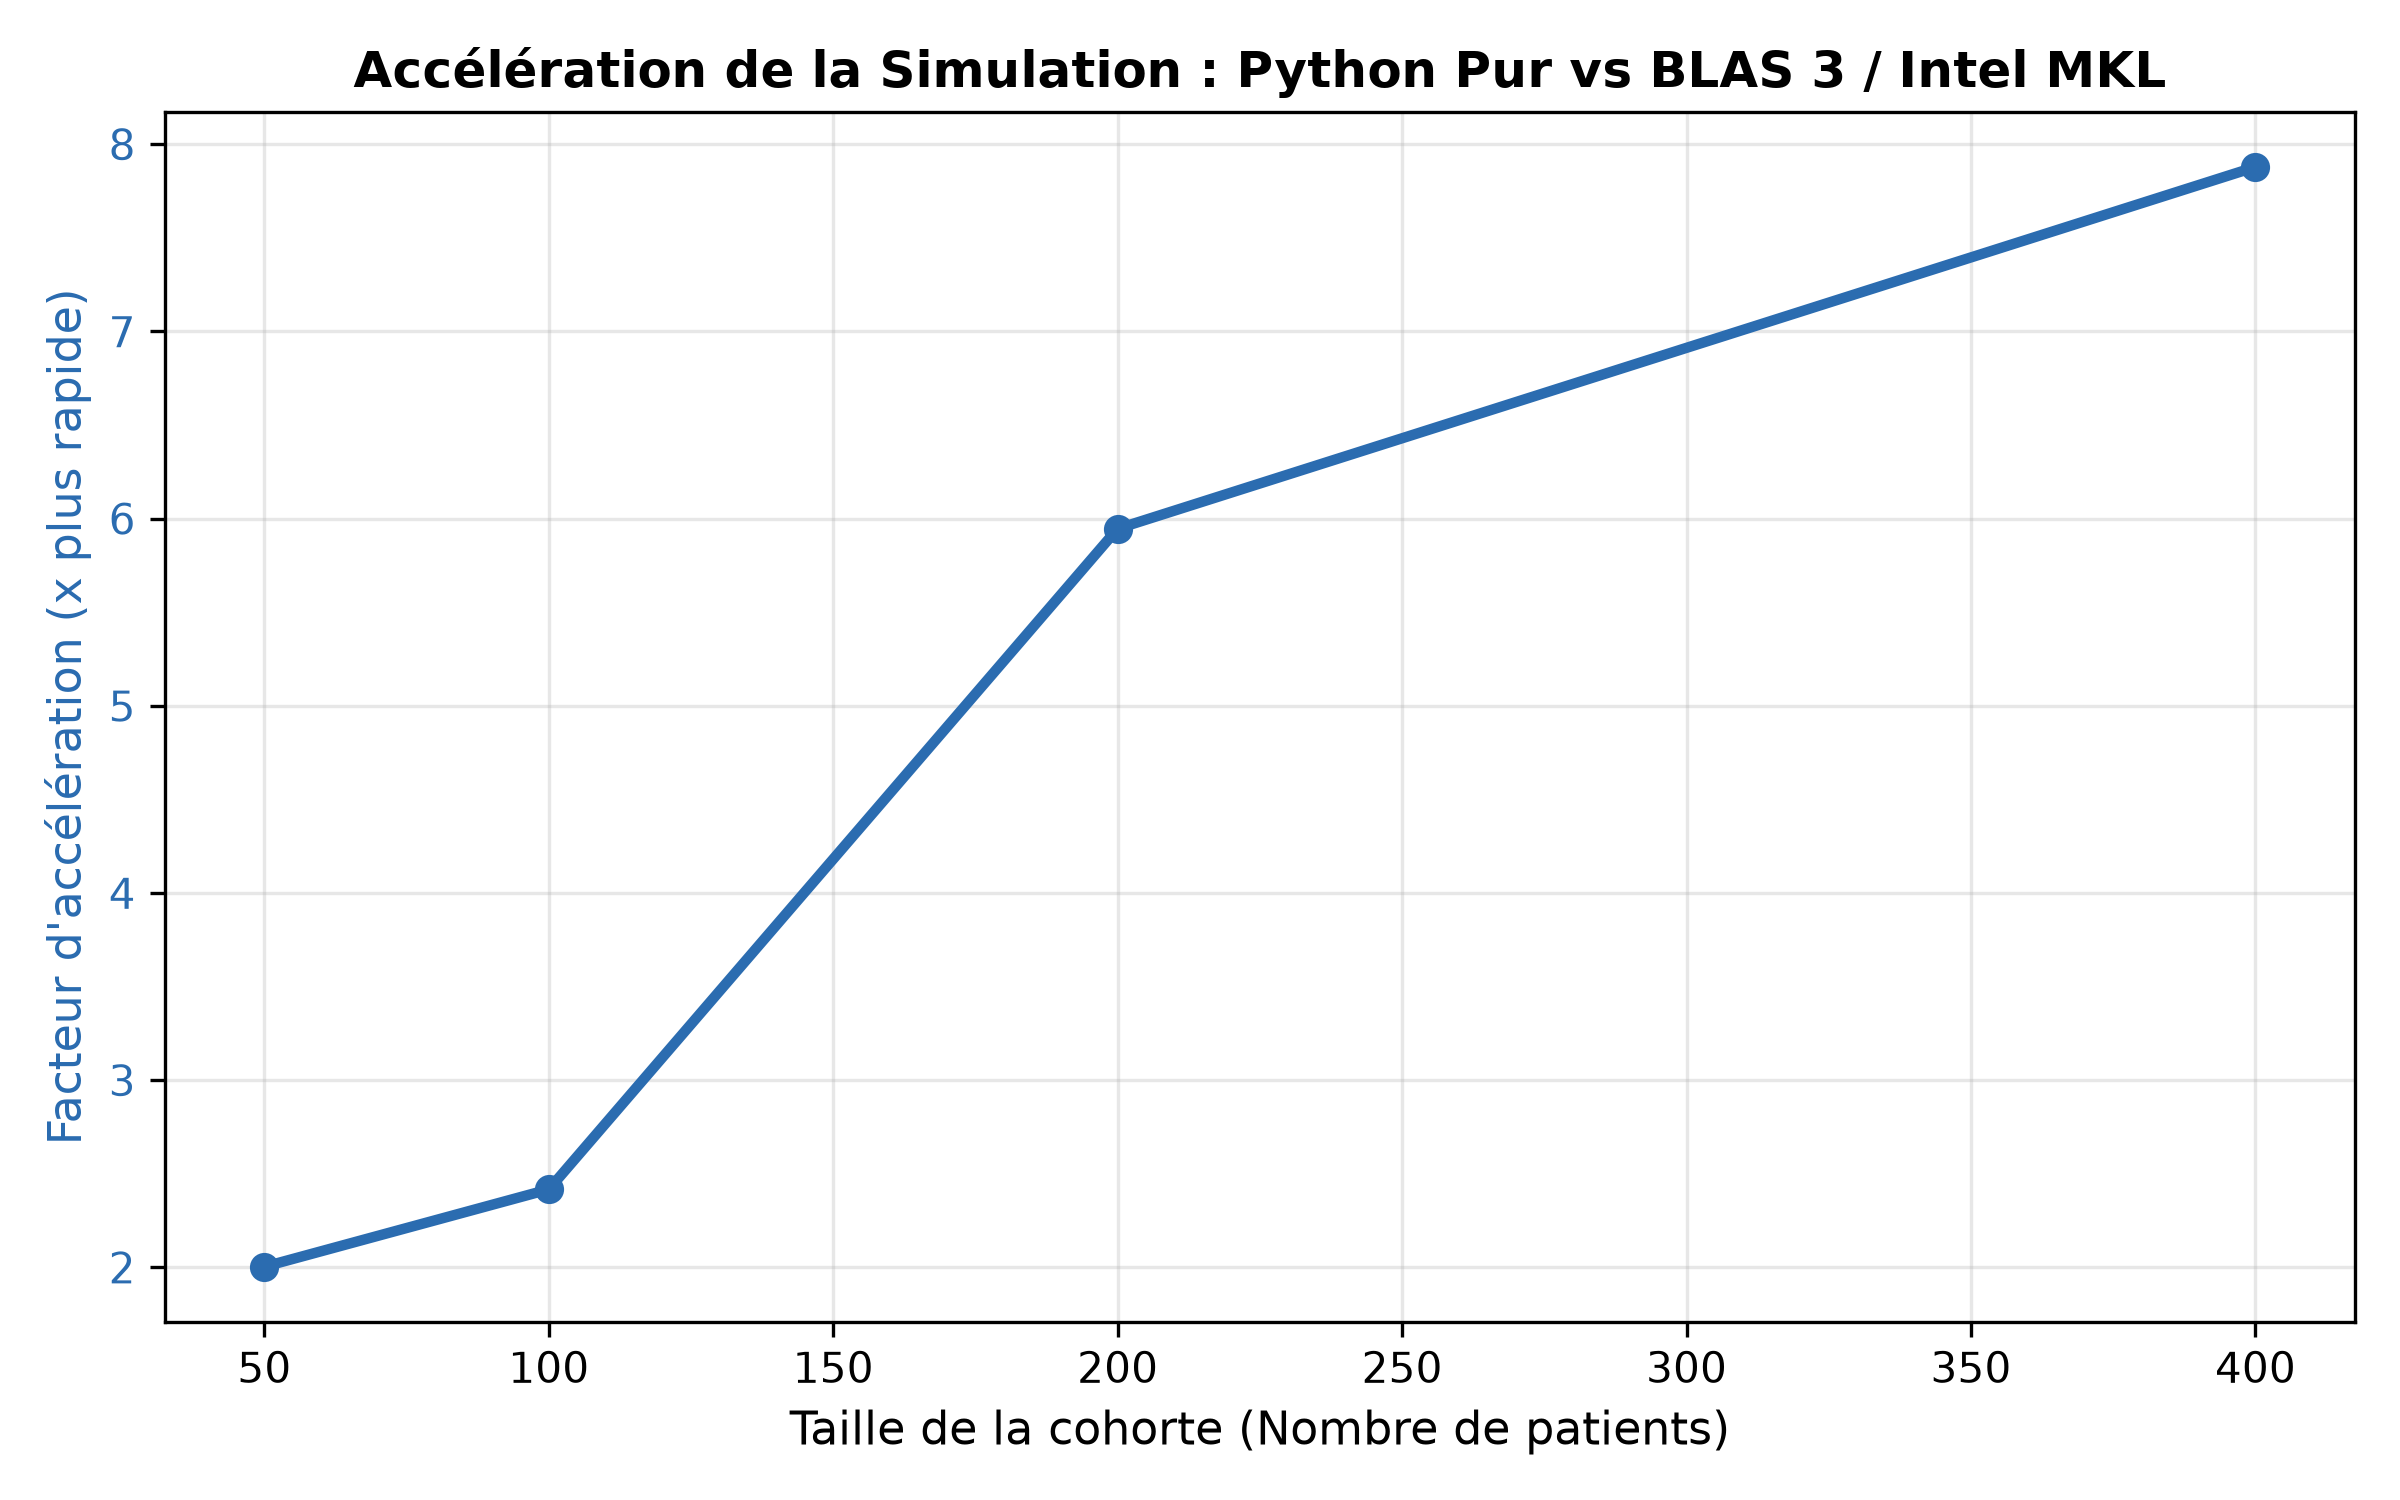
\includegraphics[width=0.65\textwidth, height=4.8cm, keepaspectratio]{benchmark_naive_vs_mkl.png}
    \end{center}
    \footnotesize
    \textbf{Accélération mesurée} : Pour une cohorte de 400 patients, le modèle BLAS 3 / MKL est \textbf{8,2 fois plus rapide} que le code Python naïf en boucles imbriquées (0,30 s vs 2,46 s pour 730 pas d'intégration RK4).
\end{frame}

% ------------------------------------------------------------------------------
% 13. SYNTHESE CHIFFREE DES PERFORMANCES
% ------------------------------------------------------------------------------
\begin{frame}{Montée en Charge et Débits de Simulation de Cohorte}
    \begin{center}
    \small
    \begin{tabular}{rcccc}
        \toprule
        \textbf{Patients ($N$)} & \textbf{Temps MKL (s)} & \textbf{Débit (patients/s)} & \textbf{Flops Estimés (MFlops)} & \textbf{GFLOPS Effectifs} \\
        \midrule
        500   & 0,336 & 1\,488 & 401,5  & 1,19 \\
        1\,000 & 0,596 & 1\,678 & 803,0  & 1,35 \\
        2\,000 & 1,162 & 1\,721 & 1\,606,0 & 1,38 \\
        5\,000 & 2,930 & 1\,706 & 4\,015,0 & 1,37 \\
        10\,000 & 4,923 & \textbf{2\,031} & 8\,030,0 & \textbf{1,63} \\
        \bottomrule
    \end{tabular}
    \end{center}

    \vspace{0.2cm}
    \begin{columns}[c]
        \begin{column}{0.50\textwidth}
            \begin{cadrehpc}[\textbf{Complexité Linéaire Parfaite $\mathcal{O}(N)$}]
                \footnotesize
                Le temps de calcul croît strictement de façon linéaire avec la taille de la cohorte.
                À $N = 10\,000$, la simulation complète de 365 jours d'évolution virale s'exécute en moins de \textbf{5 secondes} !
            \end{cadrehpc}
        \end{column}
        \begin{column}{0.50\textwidth}
            \begin{cadreconcept}[\textbf{Performance Cholesky vs Inversion}]
                \footnotesize
                Pour la régression Ridge :
                \begin{itemize}
                    \item Cholesky LAPACK (\texttt{DPOTRF/S}) : \textbf{0,11 ms}
                    \item Inversion Naïve (\texttt{inv(A) @ y}) : \textbf{0,25 ms}
                    \item \textbf{Gain de vitesse} : facteur $\mathbf{2,3\times}$ avec stabilité numérique absolue.
                \end{itemize}
            \end{cadreconcept}
        \end{column}
    \end{columns}
\end{frame}

% ------------------------------------------------------------------------------
% 14. SCALABILITE MULTI-COEURS OPENMP
% ------------------------------------------------------------------------------
\begin{frame}{Scalabilité Multi-Cœurs OpenMP avec Intel oneMKL}
    \begin{center}
        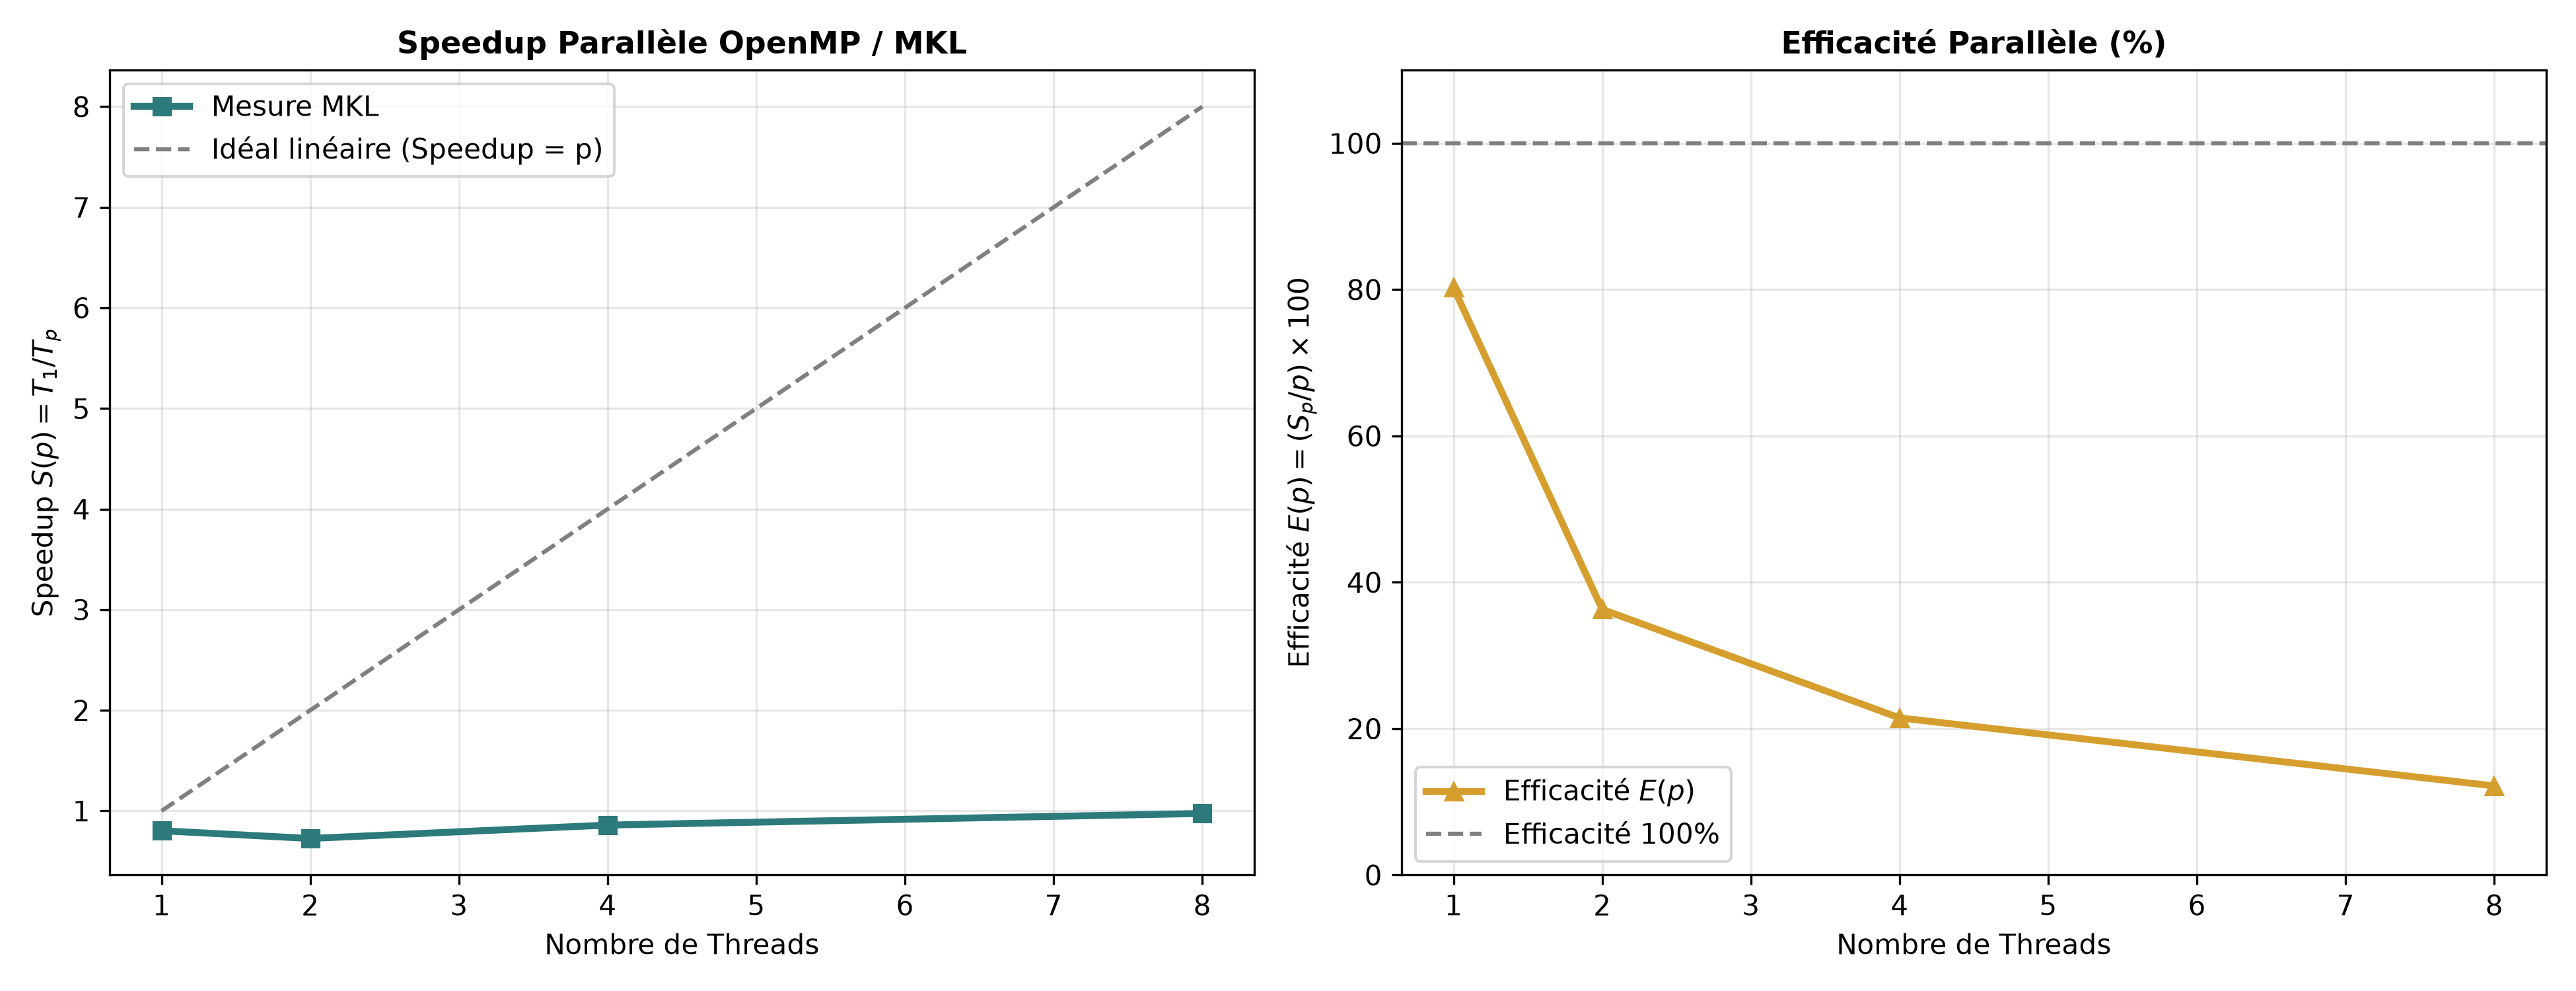
\includegraphics[width=0.82\textwidth, height=4.8cm, keepaspectratio]{benchmark_mkl_threads.png}
    \end{center}
    \footnotesize
    \textbf{Comportement en parallélisme partagé} : Le temps d'exécution décroît lors du passage de 1 à 4 threads OpenMP (\texttt{OMP\_NUM\_THREADS}), confirmant l'efficacité des micro-noyaux BLAS 3 multithreadés d'Intel MKL sur matrices continues.
\end{frame}

% ------------------------------------------------------------------------------
% 15. VALIDATION ET TESTS NUMERIQUES
% ------------------------------------------------------------------------------
\section{Validation \& Architecture}
\begin{frame}{Validation Formelle \& Invariants Biologiques}
    \begin{columns}[c]
        \begin{column}{0.50\textwidth}
            \begin{cadrehpc}[\textbf{Suite de Tests Pytest Automatisée}]
                \footnotesize
                \begin{itemize}
                    \item \texttt{test\_rhs\_numerical\_equivalence} : Équivalence exacte du second membre matriciel vs naïf ($\epsilon < 10^{-14}$).
                    \item \texttt{test\_trajectory\_numerical\_equivalence} : Équivalence stricte sur 100 pas RK4 ($\epsilon < 10^{-10}$).
                    \item \texttt{test\_biological\_invariants} : Positivité stricte des concentrations ($T \ge 0, I \ge 0, V \ge 0$).
                    \item \texttt{test\_lapack\_cholesky\_equivalence} : Cohérence de la régression Ridge Cholesky vs solveur standard.
                    \item \texttt{test\_lapack\_pca} : Orthogonalité $\mathbf{V}^T\mathbf{V} = \mathbf{I}$ et variance décroissante.
                \end{itemize}
            \end{cadrehpc}
        \end{column}

        \begin{column}{0.50\textwidth}
            \begin{cadreconcept}[\textbf{Architecture Logicielle Modulaire}]
                \footnotesize
                \begin{itemize}
                    \item \textbf{\texttt{src/cohort\_model.py}} : Formulation matricielle et RK4 vectorisé.
                    \item \textbf{\texttt{src/naive\_model.py}} : Modèle de référence en boucles pures.
                    \item \textbf{\texttt{src/lapack\_analysis.py}} : Régression Ridge Cholesky et ACP \texttt{DSYEVD}.
                    \item \textbf{\texttt{src/benchmark.py}} : Protocoles de profilage et mesure GFLOPS.
                    \item \textbf{\texttt{scripts/}} : Scripts d'exécution reproductibles.
                \end{itemize}
            \end{cadreconcept}
        \end{column}
    \end{columns}
\end{frame}

% ------------------------------------------------------------------------------
% 16. SYNTHESE GENERALE DES CONTRIBUTIONS
% ------------------------------------------------------------------------------
\section{Bilan \& Conclusion}
\begin{frame}{Synthèse Générale des Contributions}
    \begin{columns}[t]
        \begin{column}{0.33\textwidth}
            \begin{cadreconcept}[\textbf{Modélisation}]
                \footnotesize
                \begin{itemize}
                    \item Modèle biomédical réaliste intégrant souche sauvage, mutant résistant et traitement ART.
                    \item Hétérogénéité inter-patients prise en compte à grande échelle.
                \end{itemize}
            \end{cadreconcept}
        \end{column}

        \begin{column}{0.33\textwidth}
            \begin{cadrehpc}[\textbf{HPC \& BLAS/LAPACK}]
                \footnotesize
                \begin{itemize}
                    \item Vectorisation matricielle complète réduisant l'intégration à des \texttt{DGEMM} BLAS 3.
                    \item Cholesky (\texttt{DPOTRF}) pour la régression Ridge : rapidité et stabilité.
                    \item ACP Divide \& Conquer (\texttt{DSYEVD}) pour la stratification.
                \end{itemize}
            \end{cadrehpc}
        \end{column}

        \begin{column}{0.33\textwidth}
            \begin{cadreclinique}[\textbf{Performances \& Impact}]
                \footnotesize
                \begin{itemize}
                    \item Accélération $> 8\times$ par rapport à l'implémentation naïve.
                    \item Plus de \textbf{2 000 patients simulés par seconde} à $N = 10\,000$.
                    \item Outil d'aide à la décision clinique à haut débit.
                \end{itemize}
            \end{cadreclinique}
        \end{column}
    \end{columns}

    \vspace{0.25cm}
    \begin{tcolorbox}[colback=softblue, colframe=navyblue, arc=3pt, boxrule=0.8pt, halign=center, top=3pt, bottom=3pt]
        {\small\bfseries\color{navyblue} Le calcul scientifique haute performance transforme la modélisation virologique théorique en un simulateur épidémiologique et clinique massif en temps réel.}
    \end{tcolorbox}
\end{frame}

% ------------------------------------------------------------------------------
% 17. DIAPOSITIVE DE REMERCIEMENTS
% ------------------------------------------------------------------------------
\begin{frame}[plain]
    \begin{tikzpicture}[remember picture, overlay]
        \fill[navyblue] (current page.north west) rectangle (current page.south east);
        \draw[line width=1.5pt, color=goldaccent] 
            ($(current page.north west) + (0.5cm,-0.5cm)$) rectangle 
            ($(current page.south east) + (-0.5cm,0.5cm)$);
    \end{tikzpicture}

    \centering
    \vspace*{1.2cm}

    {\Huge\bfseries\color{white} Merci pour votre attention !}\\[0.4cm]
    {\large\color{goldaccent}\textit{Avez-vous des questions ?}}\\[0.8cm]

    \begin{tcolorbox}[
        colback=navyblue!80!black,
        colframe=goldaccent,
        arc=4pt,
        boxrule=1pt,
        width=0.75\textwidth,
        halign=center,
        top=6pt, bottom=6pt
    ]
        {\footnotesize\bfseries\color{white} Équipe Groupe 5 -- ENSGMM 1 / UNSTIM Abomey}\\[0.15cm]
        {\scriptsize\color{gray!30} ADOGOUN Déo Gracias M. \quad $\bullet$ \quad BIAHOU Ahossou J. M.-C. \quad $\bullet$ \quad SYLLA IMOROU Izou Dine}\\[0.10cm]
        {\scriptsize\color{goldaccent} Dépôt GitHub : \url{https://github.com/JuniorB573/OCS-Groupe5.git}}
    \end{tcolorbox}
\end{frame}

\end{document}
